% Focus on results, not on all of the theorems.
% Explain coding and decoding procedures.
% State theorems?

\chap{Polynomial Codes}{PolynomialCodes}

\section{Polynomials with coefficients in $\mathbb{Z}_2$}
\label{sec:PolynomialCodes:CoefficientsInZ2}

We are used to polynomials with coefficients that are integers or real numbers. But as we mentioned in the previous chapter, it is also possible to have polynomials with coefficients from other number systems. In this chapter, we will be looking particularly 
at the the set of polynomials with coefficients in  $\mathbb{Z}_2$: this set is denoted by $\mathbb{Z}_2[x]$.
For a polynomial in $\mathbb{Z}_2[x]$, all coefficients are either 0 or 1.

\begin{example}{}
The polynomials in $\mathbb{Z}_2[x]$ are:
\begin{enumerate}[.]
\item
The constant polynomials: 1 and 0 (there are only 2)
\item
The linear polynomials: $x$ and $x+1$ (there are only 2)
\item
The quadratic polynomials: $x^2, x^2+1, x^2 + x$,$x^2 + x+1$,
\end {enumerate}
And so on for higher-degree polynomials.
\end {example}

\begin{exercise}{}
\begin{enumerate}[(a)]
\item
How many different polynomials in $\mathbb{Z}_2[x]$ have degree 3?
\item
How many different polynomials in $\mathbb{Z}_2[x]$ have degree 4?
\item
How  many different polynomials in $\mathbb{Z}_2[x]$ have degree $n$, where $n \ge 1$?  Make a guess.
\item
Prove that your guess is correct (\emph{Hint}: Use induction, if you know how.  Otherwise, you can make a more informal argument.)
\end{enumerate}
\end{exercise}

A polynomial in $\mathbb{Z}_2[x]$ can also be represented as a \term{ binary n-tuple}\index{Binary $n$-tuple} (or binary vector) whose entries are 1's and 0's. If the degree of the polynomial is $n$, then there must be at least $n+1$ entries in the tuple.

\begin{example}{}
The polynomial $f(x) = x^3 + x^2 + x $ can be represented by the binary 4-tuple: $(1~1~1~0)$.  It can also be represented by the 5-tuple $(0~1~1~1~0)$ or the 6-tuple $(0~0~1~1~1~0)$: these representations may be useful when adding or subtracting polynomials, as we'll see in a moment.
\end{example}

Addition, subtraction and multiplication are best explained by examples.

\begin{example}{}
Let $f(x) = x^2 + x + 1$ and $g(x) = x^3   + x + 1$  be polynomials in $\mathbb{Z}_2[x]$.  We may represent $f(x)$ and $g(x)$  by the 4-tuples $(0~1~1~1)$ and $(1~0~1~1)$ respectively (note that we have used $n$-tuples of the same length: the length is determined by the highest degree of the two polynomials). Adding the polynomials is the same as adding corresponding entries of the in mod 2. It follows that the sum $f(x)+g(x)$ is:
\[\left( ~(0\oplus 1)~~~(1\oplus 0)~~(1 \oplus 1)~~~(1 \oplus 1)~\right) = (1~~1~~0~~0), \]
which corresponds to the polynomial $x^3   + x^2$. (Actually, when we represent polynomials as $n$-tuples in this way, polynomial addition is identical to addition in $\mathbb{Z}_2^n$, where $\mathbb{Z}_2^n = \underbrace{\mathbb{Z}_2 \times \ldots \mathbb{Z}_2}_{n~\text{times}}$.)

If on the other hand we take $f(x) - g(x)$, we find that we get the same answer (Try it!). This will \emph{always} be the case, because in $\mathbb{Z}_2$ addition and subtraction are the \emph{same} operation. 


\end{example}

%\begin{exercise}{}
%Multiplication is a little bit different. In this case, it's more convenient to use the polynomial representation and not resort to $n$-tuples. To multiply, we use the distributive law, tmen group terms together which correspond to the same power of $x$. So for example if $f(x) = x^2 + x + 1$ and $g(x) = x^3   + x + 1$, then:
%\begin{align*}
%f(x)\cdot g(x) &= ( x^2 + x + 1)( x^3 + x + 1)\\
%&= x^2( x^3 + x + 1) + x( x^3 + x + 1) + 1( x^3 + x + 1)\\
%&= (x^5 + x^3 + x^2) +  (x^4 + x^2 + x) + ( x^3 + x + 1)\\
%&= x^5 + x^4 + x^3 + x^3+ x^2 +   x^2 + x +  x + 1\\
%&= (x^5 + x^4 + (1\oplus 1)x^3+ (1 \oplus 1)x^2 + (1 \oplus 1)x + 1)\\
%&= (x^5 + x^4 +  1).
%\end{align*}
%\end {example}

We will be using these polynomials to represent certain special types of codes, as we shall see shortly.



\section{Cyclic Binary Codes}
\label{sec:PolynomialCodes:CyclicBinaryCodes}

  Recall from the chapter on algebraic encoding, that a code is linear if the code is determined by the null space of some matrix $H \in \mathbb{M}_{m\times n}(\mathbb{Z}_2).$\footnote{${M}_{m\times n}(\mathbb{Z}_2)$ is the set of matrices of dimension $m \times n$ whose elements are elements of $\mathbb{Z}_2$.}  So consider the codes generated by the following generator matrix:
\[
G_1 
= 
\begin{pmatrix}
1 & 0 & 0 \\
0 & 1 & 0 \\
0 & 0 & 1 \\
1 & 0 & 0 \\
0 & 1 & 0 \\
0 & 0 & 1 
\end{pmatrix}
\]
Using the methods in the previous chapter we find the resulting code words for the matrix are as follows:
\[
\begin{array}{rclccrcl}
(000) & \mapsto & (000000) & & & (100) & \mapsto & (100100) \\
(001) & \mapsto & (001001) & & & (101) & \mapsto & (101101) \\
(010) & \mapsto & (010010) & & & (110) & \mapsto & (110110) \\
(011) & \mapsto & (011011) & & & (111) & \mapsto & (111111).
\end{array}
\]

This matrix follows the typical rules of linear codes. However there is an additional interesting and useful property of these codewords.  In order to describe the property we need the following definition.

\begin{defn}{}
The \term{ cyclic 1-shift} \index{Cyclic!1-shift} of a codeword is the codeword obtained by taking the leftmost bit in the codeword and moving it to the rightmost position. The \term{ cyclic $n$-shift} \index{Cyclic!$n$-shift} of a codeword is the result of $n$ 1-shifts applied to that codeword. In the following we sometimes leave off the word ``cyclic'' for short: so ``1-shift'' means the same as ``cyclic 1-shift'', etc.
\end {defn}
According to this definition, (00101) when cyclic 1-shifted results in (01010), or when cyclic 3-shifted results in (01001).

\begin{exercise}{}
Shift the following codewords by the given cyclic shift.
\begin{enumerate}[(a)]
\item (1011)  1-shifted
\item (1010101)  1-shifted
\item (1001011)  3-shifted
\item (0101011010101) 5-shifted
\item (0101001111001)  7-shifted
\item $(z_n, z_{n-1} \cdots z_1,z_0)$  1-shifted, where $z_n \in \mathbb{Z}_2$
\item $(z_n, z_{n-1} \cdots z_1,z_0)$  3-shifted, where $z_n \in \mathbb{Z}_2$
\item $(z_{n-2}, z_{n-3} \cdots z_1, z_0, z_{n},z_{n-1})$ ($n-2$)-shifted where $z_n \in \mathbb{Z}_2$
\end {enumerate}
\end {exercise}

Now let's return to the code generated by the matrix $G_1$ given above. Notice that each cyclic 1-shift of a codeword is also a codeword.  For example, the cyclic 1-shift of the codeword $(001001)$ is $(010010)$, which is also a code word.  This is the same as stating that the set of codewords is \emph{closed} under cyclic 1-shifts.  

\begin{defn}{defcycliccode}
A linear code that is closed under cyclic 1-shifts is said to be a \term{ cyclic code}.  \index{Cyclic!code}
\end {defn}

Not all linear codes are cyclic codes.  Take the following generator matrix: 

\[
G_2 = 
\begin{pmatrix}
1 & 0 & 0 \\
1 & 1 & 0 \\
1 & 1 & 1 \\
1 & 1 & 1 \\
0 & 1 & 1 \\
0 & 0 & 1
\end{pmatrix}
\]

The resulting code words for the $G_2$ are as follows\[
\begin{array}{rclccrcl}
(000) & \mapsto & (000000) & & & (100) & \mapsto & (111100) \\
(001) & \mapsto & (001111) & & & (101) & \mapsto & (110011) \\
(010) & \mapsto & (011110) & & & (110) & \mapsto & (100010) \\
(011) & \mapsto & (010001) & & & (111) & \mapsto & (101101).
\end{array}
\]

Notice that $(101101)$ is a code word but $(011011)$ is not a code word.  Therefore the code that uses $G_2$ as a generator matrix is not a cyclic code.

Cyclic codes may be easily implemented on computers using \emph{shift registers}. Figure~\ref{fig:shift} gives some indication of how this is done for the code with generator matrix $G_1$.
\begin{figure}[h]
\begin{center}
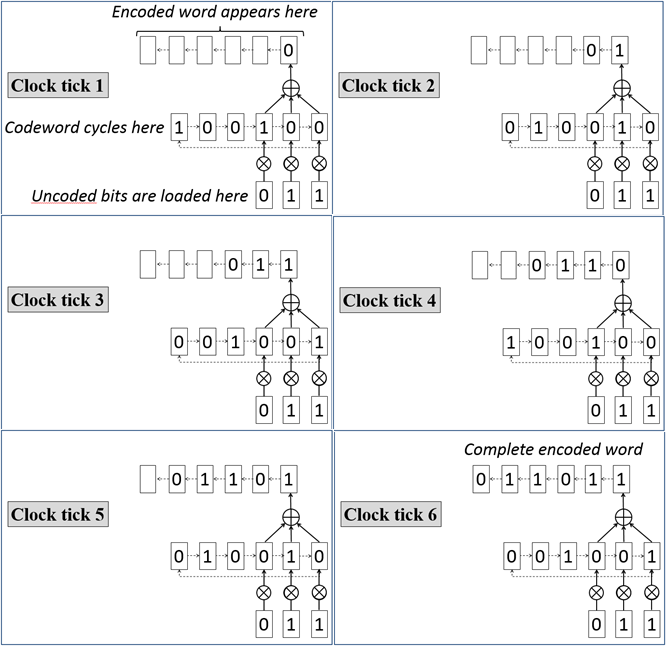
\includegraphics[width=5 in]{images/Shiftregister2.png}
\end{center}
\caption{\label{fig:shift}Shift register implementation of the code generated by matrix $G_1$. The uncoded bits are placed in the bottom ``registers" (represented by rectangles) for six ``clock ticks". At each ``clock tick", the other bits all move according to the dotted arrows. Binary multiplication and addition are performed on the bits according to the $\otimes$ and $\oplus$ symbols. }
\end{figure}

%make sure exercises include group codes that are cyclical. Low priority.
\begin{exercise}{proofofcyclic}
For each of the following sets of code words, prove or disprove that they are closed under cyclic 1-shifts.  
\begin{enumerate}[(a)]
\item
\[\begin{array}{ccccccc}
(000000) & & (111100) & & (001111) & & (110011)\\
(011110) & & (100010) & & (010001) & & (100101)
\end{array}\]
\item
\[\begin{array}{ccccccc}
(000000) & & (011100) & & (111100) & & (110011) \\
(011110) & & (100010) & & (010001) & & (101101)
\end{array}\]
\item
\[\begin{array}{ccccccc}
(000000) & & (111000) & & (000111) & & (101010) \\
(001110) & & (010101) & &(011100) & & (111111) \\
\end{array}\]
\end {enumerate}
\end {exercise}

\begin{exercise} {}
\begin{enumerate}[(a)]
\item
Prove or disprove: A cyclic code is closed under cylic $2$-shifts.
\item
Prove or disprove: A cyclic code is closed under cylic $3$-shifts.
\item
Prove or disprove: A cyclic code is closed under cylic $n$-shifts for any $n \in \mathbb{N}$. (Use induction if you can--otherwise, you may make a more informal argument.)
\end{enumerate}
\end {exercise}

\begin{example}{cyclic_poly}
An interesting (and sometimes useful) property of some binary codes is that the reverse of each codeword is also a codeword. 
Take for example the following cyclic  code of length 4 :
 \[S = \{(0000),(1010),(0101),(1111)\}\]  
The codewords $(0000)$ and $(1111)$ read the same backwards and forwards: such codewords are called \term*{palindromic}\index{Codeword!palindromic}\index{Palindromic!codeword}. The remaining two codewords $(1010)$ and $(0101)$ are reverses of each other. Thus the reverse of every codeword in $S$ is also a codeword in $S$.

Codes for which the reverse of every codeword is a codeword are called \term*{reversible codes}.\index{Code!reversible}\index{Reversible code}  Such codes are interesting because they can be read either backwards or forwards (although the forward and backward readings will be different!), and are useful in certain data storage applications\footnote{See Massey, J. L. (1964). ``Reversible codes''. \textit{Information and Control}, 7(3), 369-380.}.  
\end {example}

\begin{exercise}{}
\begin{enumerate}[(a)]
\item
Give an example of a binary code that is not reversible.
\item
Show that all cyclic codes of length 2 and 3 are reversible codes.
\item
Show that all cyclic codes of lengths 4 are  reversible codes. (\emph{Hint}: How many code words are palindromic? You don't need to check these.  The remaining code words divide into pairs, where the two code words in a pair are reverses of each other. You just need to show that the two code words in each pair are cyclic shifts of each other.) 
\item
*Show that all cyclic codes of length 5 are  reversible codes. (\emph{Hint}:  You will need to use the cyclic codes are defined to be linear.)
\end{enumerate}
\end{exercise}

\begin{exercise}{}
Let $S$ be a binary cyclic code, and suppose that $S$ contains a palindromic codeword $w$. Show that the reverse of every cyclic shift of $w$ is also a cyclic shift of $w$.
\end{exercise}

\begin{exercise}{}
Suppose a code $C$ has a generator matrix $G$ with two columns, such that the two columns are reverses of each other. Show that $C$ is a reversible code.
\end{exercise}

\begin{exercise}{}
Suppose a code $C$ is reversible, and has an odd number of codewords. Prove that at least one codeword in $C$ is palindromic.  Is it possible that $C$ could have exactly two codewords are palindromic in this case?  
\end{exercise}


% Show that if n is odd and cyclic code contains two codewords that are mirror images of each other, then at least one codeword is a palindrome.
% Show that cyclic codes divide the set of all codewords into equivalence classes.  (Not quite true -- must be generated by a single codword).
% Show that the number of distinct cyclic codes is greater than 2^n/n
% Show tha tthe number of palindromes is 2^ceil(n/2)
% Show that if 2^ceil(n/2) > n and n is odd, then there must exist a cyclic code that is not a reversible code

\section{Polynomial Codes: definition and basic properties}
\label{sec:PolynomialCodes:DefinitionAndProperties}

In Section~\ref{sec:PolynomialCodes:CoefficientsInZ2} we mentioned that  any polynomial in $\mathbb{Z}_2[x]$ can be written as a binary $n$-tuple: for example, the polynomial $x^6 + x^4 + x$ would be represented as $(1010010)$ . Notice that in the $n$-tuple, the coefficient of the highest order term is on the \emph{left}, and the coefficient of the lowest-order term written on the \emph{right}.  We did this because this is how you write polynomials in high school or college algebra.  However, the reader should take note that many references on polynomial codes  \emph{reverse} this order, and list the lowest-order coefficient on the \emph{left}.

Now we'll turn the relationship around. Any list or vector of binary digits, similar to the code words in the previous section, can be represented as a polynomial. For example $(101101)$ can be represented as the polynomial $1x^5 + 0x^4 + 1x^3 + 1x^2 + 0x + 1 = x^5 + x^3 + x^2 + 1$.  

\begin{exercise}{}
Suppose a vector contains 10 binary digits (binary digits are also referred to as \term{bits}).
\begin{enumerate}[(a)]
\item
 What is the highest possible degree of the polynomial corresponding to the vector?
\item
If the degree of the corresponding polynomial is 6, what can you say about the vector?
\item
If the corresponding polynomial has only even powers of $x$, what can you say about the vector?
\end{enumerate}
\end{exercise}

Recall that we have defined a code of length $n$ (or $n$-bit code) as a set of binary $n$-tuples.  We can use polynomials to generate codes as shown in the following example. 

\begin{example}{}
Let $p(x) = x^3 + 1$.  Consider all polynomials of degree $\le$ 2: they are \[0, 1, x, x+1, x^2, x^2+1, x^2 + x, x^2 + x + 1.\]  Take $p(x)$ times each of these polynomials and represent the results as binary 6-tuples:

\begin{align*}
0\cdot p(x))&=0x^5+0x^4+0x^3+0x^2+0x+0=(000000),\\
1\cdot (p(x))&= x^3 + 1=(001001),\\ 
x(p(x))&=x^4+x= (010010),\\
x^2(p(x))&=x^5+x^2=(100100),\\
(x+1)p(x)&=(010010)+(001001)=(011011),\\
(x^2+1)p(x)&=(100100)+(001001)=(101101),\\ 
(x^2+x)p(x)&=(100100)+(010010)=(110110), \textrm{and}\\
(x^2+x+1)p(x)&=(100100)+(010010)+(001001)=(111111).
\end{align*}

So we have the following set:
 \[ \begin{array}{cccc}
(000000) & (100100) & (001001) & (101101) \\
(010010) & (110110) & (011011) & (111111).
\end{array}\]
We call this set of codewords the code of length 6 (or 6-bit code) generated by $p(x)$.
\end {example}

We generalize this example with the following definition.

\begin{defn}{polynomialcode}
Let $p(x)$ be a polynomial of degree $d$ with coefficients in $\mathbb{Z}_2$ and $S$ be the set of all polynomials in $\mathbb{Z}_2[x]$ with  degree $m$ or less. The \term*{ polynomial code generated by $p(x)$}\index{Polynomial code!generated by a polynomial} \term*{of length} $d+m+1$  is the subset of $\mathbb{Z}_2^{d+m+1}$ corresponding to the set of products of $p(x)$ with each polynomial in $S$. 
\end {defn}

\begin{exercise}{}
Find the 7-bit codes generated by the following polynomials.
\begin{enumerate}[(a)]
\item $x^5 + x^3 + x^2 + 1$
\item $x^4 + x^3 + x$
\item $x^5 + x^4 + x^2 + x$
\item $x^4 + x^2$
\end {enumerate}
\end {exercise}
%
%\begin{solution}{}
%\begin{enumerate}[(a)]
%\item $(0000000), (0101101), (1011010), (1110111)$
%\item $(0000000), (0011010), (0110100), (0101110), (1101000), (1110010), (1011100),(1000110) $
%\item $(0000000), (0110110), (1101100), (1011010)$
%\item $(0000000), (0010100), (0101000), (0111100), (1010000), (1111000), (1010100), (1111100)$
%\end {enumerate}
%\end {solution}

\begin{exercise}{}
Find the 5-bit codes generated by each of the following polynomials: 
\begin{enumerate}[(a)]
\item $x + 1$
\item $x^3+x+1$
\item $x^2 + x$
\end{enumerate}
\end {exercise}


In our previous discussion of binary codes in Chapter~\ref{ErrorAndCorrectionCode}, we made a big deal about \emph{linear codes}.  Recall that a linear code is a code that is closed under addition:  

\begin{exercise}{lincode}
Show that the following code is a linear code
\[\{(0000),(1010),(0101),(1111)\}\]
\end {exercise}

Notice that in Exercise~\ref{exercise:PolynomialCodes:lincode}, we used the cyclic polynomial code from Example~\ref{example:PolynomialCodes:cyclic_poly}.  Therefore it is possible for a polynomial code to be a linear code.  But are all polynomial codes linear codes? That's the million-dollar question. Let's explore a bit:


\begin{exercise}{}
Let $p(x) = x^3 + x + 1$, let $G_1$ be the set of 6-tuples that are multiples of $p(x)$.
\begin{enumerate}[(a)]
\item
Show that $(100111)$ and $(010110)$ are multiples of 
$p(x)$.
\item
Show that $(100111)+(010110)$is a multiple of $p(x)$. (Here `+' is in the sense of $\mathbb{Z}_2[x]$.)
\item
Show that the polynomial code consisting of multiples of $p(x)$ is a linear code (that is, it is closed under addition).
\end{enumerate}
\end{exercise}

The preceding exercise is not a general proof, but it is possible to generalize the method used to show that polynomial codes are indeed linear codes. It's actually not difficult to obtain the generator matrix for a given polynomial code, as the following example shows.

\begin{example}{}
Consider the $(6,3)$ code corresponding to the polynomial $x^3+1$.  We therefore have
\begin{align*}
&1 \text{ encodes as }x^3+1,\\
&x \text{ encodes as }x^4+x,\\
&x^2 \text{ encodes as }x^5+x^2.
\end{align*}
All of the above polynomials also have $n$-tuple representations.  Using $n-tuples$, the same encoding information can be written as
\[
\begin{array}{rcl}
(001) & \mapsto & (001001),  \\
(010) & \mapsto & (010010) , \\
(100) & \mapsto & (100100). \\
\end{array}
\]

To obtain the generator matrix, we simply write the codewords for $(100), (010),$ and $(001)$ as column vectors next to each other.

\[\begin{pmatrix} 
1 & 0 & 0\\
0 & 1 & 0\\
0 & 0 & 1\\
1 & 0 & 0\\
0 & 1 & 0\\
0 & 0 & 1\\
\end{pmatrix}\]

Since the smallest weight of any of the nonzero codewords is 2, this code has the ability to detect all single errors.  

\end {example}

\begin{exercise}{}
Give the generator matrix for the codes generated by the following polynomials.
\begin{enumerate}[(a)]
\item The (5,3) code generated by $x^2 + x$.
\item The (7,4) code generated by $x^3 + x $.
\item The (9,5) code generated by $x^4 + x^2 + 1$.
\end {enumerate}
\end {exercise}

%\section{Polynomial Properties}
%
%Now for polynomials to work as an encoding algorithm, we need to define a few things about the polynomials.  As demonstrated above, the coefficients of a polynomial used in encoding are members of $\mathbb{Z}_2$.  That is all coefficients of the indeterminates must be 0 or 1. Another way to represent this is all operations on the polynomials are performed $\pmod{2}$.  This yields a limited list of polynomials that can be used.
%
%\footnote {This section relies heavily on material from source}
%%DLW, need to insert a reference to Cooper here 10/31/2012.
%
%
%Now division of polynomials we need to approach carefully.  Recall the division algorithm states that for and 2 integers $j$ and $k$ where $k$ is not 0, there are uniqe values $q$ and $r$ such that $k = j \cdot q + r$ where $q$ and $r$ are integers and $r < j$. The same rule applies for dividing polynomials.  Given polynomials in $f(x)$ and $g(x)$. There exist unique polynomials $q(x)$ and $r(x)$ such that $f(x) = g(x)\cdot q(x) + r(x)$ where $r(x)$ must be "smaller" than $g(x)$.  In the case of polynomials, this smaller is represented by a smaller degree.  Therefore the degree of $r(x)$ must be smaller than the degree of $g(x)$.  The polynomial $q(x)$ is called the \term{ quotient} and the polynomial $r(x)$ is called the \term{ remainder}.\index{Quotient} \index{Remainder}  Now the reason we need to be careful with polynomial division is that one polynomial divided by another is not a polynomial unless the remainder polynomial $r(x)$ is the 0 polynomial.  When the remainder of a polynomial division is 0, we say that $g(x)$ divides $f(x)$.
%
%\begin{example}{}
%A quick reminder of the process of dividing polynomials.
%
%$g(x) = x^2 - x + 12$ divided into $f(x) = 5x^3 - x^2 + x$ 
%
%
%multiplying $g(x)$ by $5x$ results in:$5x^3 - 5x^2 + 60x$, subtract from $f(x)$ to get:
%\[4x^2 -59x\]
%Then multiply $g(x)$ by $4$ to get $4x^2 -4x + 48$ and subtract from $4x^2 -59x$ to get:
%\[-55x - 48\]
%
%We can write this as $5x^3 - x^2 + x = (5x+4)\cdot(x^2 - x + 12) + (-55x - 48)$
%\end {example}
%
%\begin{example}{}
%Dividing polynomials in $\mathbb{Z}_2$ is very similar.  Given $x^2 + 1$ divided by $x+1$
%
%We see that $x+1$ goes into $x^2 + x + 1$ a total of $x$ times yielding $x^2 + x$ which yields a remainder of $-x + 1$.  Then, $x+1$ goes into the remainder $-1$ times with a remainder of $2$.  The remainder is then taken ${\pmod 2}$ to yield a remainder of 0.  So in $\mathbb{Z}_2$, $x^2+1$ is evenly divisible by $x+1$.
%
%\end{example}

%The remainder theorem. 
%Consider moving this to poly_rings.
%\begin{prop}{polyremainder}
%When dividing $f(x)$ by $x-a$, the remainder is $f(a)$.
%\end {prop}
%
%\begin{proof}
%By the division algorithm above, if we divide $f(x)$ by $x-a$, it will produce two unique polynomials $q(x)$ and $r(x)$ such that $f(x) = (x-a)q(x) + r(x)$.  Since the degree of $x-a$ is 1, then according to the division algorithm, the degree of $r(x)$ must be less than 1.  Therefore $r(x)$ has to be a constant.  We will show this replacing $r(x)$ with $r$ where $r$ is an real number.  This yields:
%\[f(x) = (x-a)q(x) + r\]
%If we set $x=a$ then we get:
%\[f(a) = (a-a)q(x) + r \rightarrow f(a) = 0 \cdot q(x) + r \rightarrow f(a) = r\]
%\end {proof}
%
%The following proposition in an important special case of Proposition~\ref{proposition:PolynomialCodes:polyremainder}.
%
%\begin{prop}{}
%$a$ is a root of $f(x)$ if and only if $x-a$ divides $f(x)$.
%\end {prop}
%
%From Proposition~\ref{proposition:PolynomialCodes:polyremainder} $f(x) = (x-a)\cdot q(x) + f(a)$, so $f(a) = 0$ if and only if $f(x)=(x-a)\cdot q(x)$ which is true if and only if $x-a$ divides $f(x)$.
%
%%irreduceable polynomials
%It is possible for a polynomial to always have a remainder regardless of which polynomial is used to divide it.  A polynomial that cannot be evenly divided cannot be further factored.  A polynomial that cannot be further factored we call an \term{ irreducible polynomial}.  \index{Irreducible Polynomial} These polynomials serve a similar function for polynomials as prime numbers do for integers.  Since these polynomials cannot be reduced, we can make deductions as to the behavior of a product of irreducible polynomials.  For example the polynomial $(x+a)$ where $a$ is a real number cannot be factored any further, and the polynomial $mx+b$ where $m$ and $b$ are reals can only be factored into $(x+b/m)(m)$.  A like with real numbers, if we know that $f(x) \cdot g(x) = 0$ then either $f(x) = 0$ or $g(x) = 0$.  Now it is possible to get a higher degree polynomial to be irreducible, but the number set that is used can affect the irreducibility of a polynomial.  For example $x^2 + 1$ is irreducible over the reals, but could be factored over the complex numbers into $(x-i)(x+i)$.  

%Start the arguments of cyclic codes in polynomials.  

We now have enough information to approach the question of when a polynomial code is a cyclic code.  We must first define a cyclic shift in terms of polynomials.  We understand to perform a cyclic shift on an $n$-tuple, we just take the left most digit in the $n$-tuple and put it on the right of the $n$-tuple.  $(1011)$ would turn into $(0111)$.  However moving the terms of a polynomial does not change its value.  In this case we have to multiply the whole polynomial by $x$ to shift the terms up a degree, but there is an additional step needed to move the highest term to the lowest.  To do this, we have to use modular polynomial division.  

\begin{example}{}
The $n$-tuple (0111) when cyclically shifted once, results in (1110).  So the polynomial $p(x) = x^2 + x + 1$ when cyclically shifted once is $x^3 + x^2 + x$.  When we multiply $p(x)$ by $x$, we get $x^3 + x^2 + x$.  In this case, multiplication by $x$ gives the cyclic shift.

The $n$-tuple (1011) when cyclically shifted once results in (0111).  So the polynomial $p(x) = x^3 + x + 1$ when cyclically shifted once is $x^2 + x + 1$.  We multiply $p(x)$ by $x$ to yield $xp(x) = x^4 + x^2 + x$, which is not the same codeword as (0111).  Therefore, we must divide by $x^4 + 1$.
\[x^4 + x^2 + x = 1\cdot (x^4 + 1) + (x^2 + x - 1)\]
and the last term $-1$ gets taken $\pmod 2$ to yield.
\[x^2 + x + 1\]
Which is the same as the $n$-tuple (1110).
\end{example}

\begin{prop}{cyclicremainder}
A cyclic shift of a $n$-bit polynomial codeword $p(x)$ is the same as multiplying the codeword $p(x)$ by $x$ then taking the remainder after dividing by $x^n + 1$.
\end{prop}

\begin{proof}{}

\term{ Case 1:}
The polynomial codeword has a degree of less than $n-1$. In this case, a polynomial of the form $p(x)= 0x^{n-1} + a_{n-2}x^{n-2} + a_{n-3}x^{n-3} \cdots + a_{1}x + a_0$ where $a_n \in \mathbb{Z}_2$, when multiplied by $x$ would result in $xp(x)=a_{n-2}x^{n-1} + a_{n-3}x^{n-2} \cdots + a_1x^2 + a_{0}x + 0$ Which is the cyclically shifted code word.  Then when taking the remainder after division by $x^n + 1$, we notice that the degree of $x^n + 1$ is larger than $xp(x)$, so the quotient must be 0 and the remainder will be $xp(x)$.

 
\term{ Case 2:}
The polynomial codeword has a degree equal to $n-1$.  In this case, a polynomial of the form $p(x)= a_{n-1}x^{n-1} + a_{n-2}x^n-2 + a_{n-3}x^n-3 \cdots + a_{1}x + a_0$, where $a_n \in \mathbb{Z}_2$, when multiplied by $x$ would result in $xp(x)=a_{n-1}x^n + a_{n-2}x^{n-1} \cdots + a_1x^2 + a_{0}x + 0$.  This is close to the cyclically shifted codeword, but has an $x^n$ term that is not in any codeword.  We then divide by $x^n + 1$, since both $xp(x)$ and $x^n + 1$ have a $x^n$ term, the quotient is 1.  Then taking the remainder will yield, $a_{n-2}x^{n-1} \cdots + a_1x^2 + a_{0}x - 1$.  But remember we're doing arithmetic in $\mathbb{Z}_2$, so $-1 = 1$.  Thus the remainder is $a_{n-2}x^{n-1} \cdots + a_1x^2 + a_{0}x + 1$ which is the cyclically shifted codeword.
\end{proof}

\begin{exercise} {cycShift}
For the following polynomials, calculate their cyclic shift by multiplying by $x$ then taking the remainder after division of $x^n + 1$.
\begin{enumerate}[a]
\item
$x^3 + x^2 + 1$ where $n=4$
\item
$x^7 + x^4 + x^2$ where $n=8$
\item
$x^9 + x^8 + x^7 + x^5 + x^4 +x^2 + 1$ where $n=10$
\end {enumerate}
\end {exercise}

\begin{prop}{cyclicsum}
Any cyclic shift of $p(x)$ can be written as a sum of $p(x) + q(x)(x^n + 1)$, where $p(x)$ is a codeword and $q(x)$ is some polynomial.  
\end {prop}

\begin{proof}
Given a $n$-bit codeword $p(x)$, the cyclic shift of $p(x)$ is calculated by $xp(x) = q(x)(x^n + 1) + r(x)$ where $q(x)$ is some polynomial and $r(x)$ is a polynomial of degree less than $n$.  Simply subtract $q(x)(x^n + 1)$ from both sides to yield $xp(x) - q(x)(x^n + 1) = r(x)$.
\end {proof}

%Up to now, we have only discussed cyclic shifts that move the codeword one space.  In order for a code to be a cyclic code, shifts of any length must be codewords.  For cyclic shifts larger than 1, we have the following.
%
%
%\begin{prop}{}
%Suppose $C$ is a code such that any codeword $c(x)$ when cyclically shifted by 1 is a codeword. Then $C$ is a cyclic code.
%\end {prop}
%\begin{proof}
%Given a code $C$ and an arbitrary codeword $c(x)$ such that the cyclic shift by 1 of $c(x)$ is a code word, an arbitrary shift of $n$ spaces is nothing more than $n$ cyclic shifts of 1.  Therefore an arbitrary shift must also be a codeword.
%\end {proof}

We next introduce the notion of a complete polynomial, which resembles the idea of a generator of a cyclic group.\footnote{In fact, a complete polynomial IS the generator of a group of nonzero polynomials under multiplication.} 

%Complete polynomials
\begin{defn}{defn:Completepolynomials}
A\term{ complete polynomial} \index{Complete polynomials} is a polynomial $f(x)\in \mathbb{Z}_2[x]$ of degree $n$ such that for every nonzero polynomial $g(x)\in \mathbb{Z}_2[x]$ of degree $n$ or less, there exists a positive integer $k$ such that $g(x)-x^k$  is divisible by $f(x)$.
\end{defn}

\begin{example}{}
The polynomial $x^3 + x + 1$ is complete.  First, we set the equation equal to 0. $x^3 + x + 1=0$ Add $x+1$ from both sides to yield: $x^3 = x+1$. (Remember, addition is the same as subtraction in $\mathbb{Z}_2[x]$.) Multiply by $x$ to get
\[x^4 = x^2 + x,\]
and again to get
\[x^5 = x^3 + x^2.\] 
Now substitute $x+1$ for $x^3$ to get $x^5 = x + 1 + x^2$. Multiply again by $x$ to yield.
\[x^6 = x^3 + x^2 + x,\]
and substitute again for $x^3$ to get (after some algebra)
\[x^6 = x^2 + 1\]
Multiply once more by $x$ to get $x^7 = x^3 + x = 1.$

So if we list the possible polynomials of degree 2 or less, each is paired to a power of $x$.
\[
\begin{array}{lcr}
x^0 & = & 1 \\
x^1 & = & x \\ 
x^2 & = & x^2 \\ 
x^3 & = & x+1 \\ 
x^4 & = & x^2 + x \\ 
x^5 & = & x^2 + x + 1 \\ 
x^6 & = & x^2 + 1 \\ 
x^7 & = & 1 
\end{array}\]
Therefore the polynomial $x^3 + x + 1$ is complete for polynomials of degree 2 or smaller.  
\end {example}

%Insert a note connecting complete polynomials to cyclic codes.

With these properties in place, we can now show how to generate a cyclic code with polynomials.  

\begin{example}{}
Let $p(x)$ be $x+1$ and $f(x) = x^5 + 1$ be a polynomial to be encoded.  The product of the two would be the codeword $f(x)p(x) = x^6 + x^5 + x + 1$.  To cycle the codeword left, we would need to multiply by $x$. This would yield $x^7 + x^6 + x^2 + x$.  However, since this is a 7-bit code, there is no place for an $x^7$ term.  So we need to shift the $x^7$ term to an $x^0$ term.  This is done by 
taking the remainder after dividing by $x^7+1$.  

$x^7 + 1$ goes into $x^7 + x^6 + x^2 + x$ once, this cancels the $x^7$ term and has $x^6 + x^2 + x - 1$ as the remainder, but remember that this operation is done $\pmod 2$ so the remainder is $x^6 + x^2 + x - 1$.  $x^7 + 1$ does not divide any further as all the remaining terms are of a lesser degree.  
This new term we can then divide by $x+1$ to show that it is in the code.  $x+1$ goes into $x^6 + x^2 + x + 1$ exactly $x^5 + x^4 + x^3 + x^2 + 1$ times $\pmod2$.  We can continue multiplying by $x$ and taking the remainder after division by $x^7 + 1$ to generate additional codewords.

So for the 7-bit polynomial code generated to be cyclic, $p(x)$ must divide $x^7 + 1$.  Using polynomial division we can show that $x^7 = (x+1)(x^6-x^5+x^4-x^3+x^2-x+1) + 0$.  So $p(x)$ divides any product of $x^7+1$.

We can show that $x+1$ divides $x^n + 1$.  First lets show that $p(x)$ divides $x^2 + 1$.  $(p(x))^2 = x^2 + 2x + 1$, but remember $2x = 0$ in $\mathbb{Z}_2$ so $(p(x))^2 = x^2 + 1$. Likewise we can show that $x+1$ divides $x^3 + 1$.  Using polynomial multiplication, we can show that $(x+1)(x^2 -x + 1) = (x^3 + 1)$.  However we need to show that $x+1$ divides $x^n+1$ for any $n$.
\end {example}

\begin{prop}{}
If a polynomial $p(x)$ divides $x^n + 1$, then the $n$-bit polynomial code generated by $p(x)$ is cyclic.
\end {prop}

\begin{proof}{}
Let $C$ be the code generated by $p(x)$, and let $f(x)$ be an arbitrary codeword in $C$.  Then by Definition~\ref{definition:PolynomialCodes:polynomialcode}, $f(x)= a(x)p(x)$.  Let $g(x)$ be the cyclic shift of $f(x)$ by $1$. By Proposition~\ref{proposition:PolynomialCodes:cyclicremainder}, $g(x)$ is the remainder of  $xf(x)$  when divided by $x^n+1$.  By Proposition~\ref{proposition:PolynomialCodes:cyclicsum},  $g(x)=xf(x) +  q(x)(x^n + 1)$. Since $p(x)$ divides $x^n+1$, then $x^n+1=s(x)p(x)$.  By substitution, $g(x)=xa(x)p(x) +  q(x)s(x)p(x)=p(x)\bigg(xa(x)+  q(x)s(x)\bigg)$. Therefore, $g(x)$ is a multiple of $p(x)$: in other words, $g(x)$ is in the code generated by $p(x)$, which is none other than $C$. We have thus shown that any cyclic shift of an arbitrary codeword in $C$ is also in $C$. This is exactly what it means for the code $C$ to be a cyclic code. Thus the proposition is proved.
\end{proof}

%If a polynomial p(x) divides x^n + 1, then the n-bit polynomial code generated by p(x) is cyclic, because any codeword that can be shifted is a multiple of (x^n+1). Include example in written notes.

%exercise prove x^n+1 always divides x^(mn) + 1 in z2


%Any n-bit cyclic code is generated by a polynomial that divides x^n + 1  (this one is harder to prove -- basically, given two codewords in the code you need to show that the gcd is also in the code.  The proof is similar to the Euclidean algorithm. It follows that the gcd of all codewords must generate the code)  [[ Go back to polynomials chapter and add an example showing the gcd of two polynomials in Z_2[5] after example 3.6.30.

%Want to show that each remainder is unique so that we can detect errors.  Each single bit error will decode differently.
%Suppose that x does not divide p(x). Then two different powers of x (x^n and x^m) have the same remainder under division by p(x) if and only if p(x) divides x^(n-m) + 1  (since p(x) must divide x^n - x^m, which is the same as x^m*(x^(n-m) + 1), and by unique factorization the factors of p(x) must all divide (x^(n-m) + 1).  This proof requires unique factorization of polynomials).

%keep taking x^n mod p(x) for larger n, since p(x) is a prime polynomial then x^n for some value of n means x^n = 1 mod p(x).  => x^n -1 = 0 mod p(x) => p(x) divides x^n -1.  Since the coefficient are in z2 => p(x) divides x^n + 1.
%(4) Every prime polynomial p(x) (i.e. polynomial that has no factors) divides x^n + 1 for some value of n (since the nonzero remainders under division by p(x) form a multiplicative group G, therefore the polynomial x must have finite order so there must be some power of n such that x^n = 1 under multiplication mod p(x)).


%The gcd of all the codewords is the smallest degree polynomial that can be derived from a linear combination and it is true that it must divide all the polynomial codewords.  List as part of the process. (medium to low priority) write a proof.


%The order of an element, must divide the order of the group.
%5) Let n be the smallest positive integer such that p(x) divides x^n + 1  (n is finite by (4)). Then n <= 2^(m+1)-1  (since the order of x in G [defined in (4)] must be less than or equal to the order of G, which is 2^(m+1) - 1. M is the degree of p(x).


%(6) Suppose p(x) is a polynomial of degree m, and the smallest n such that p(x) divides x^n+1 is 2^(m+1) - 1. Then 1,x,...x^[2^(m+1)-2] all have distinct remainders when divided by p(x). 


